\chapter{Experiments and Evaluation Framework (12)}
\label{chp:experiments_and_framework}
Warum

Wie

Mit welchem Forschungsdesign
Welches ist das Forschungsartefakt, mit dem in dieser Thesis gearbeitet wird?

\section{Research Process}
This chapter describes the practical implementation of the research presented in this thesis. Starting from raw operational data obtained from HHLA Container Terminal Burchardkai, an event log is engineered and enriched with contextual information. The resulting event log serves as the foundation for process discovery and simulation discovery. Subsequently, a series of simulation experiments are conducted and evaluated using the similarity metrics introduced in Chapter~\ref{chp:background}.
[IMAGE TO BE DESCRIPTED]

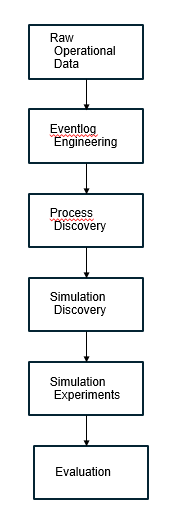
\includegraphics{figures/schemas/ResearchDesignV1.png}



\section{Case Study Environment}
\texit{define the research object}
HHLA

Terminal
Truck Process
\subsecton{IT Landscape}
The operational data used in this thesis originate from multiple information systems that support day-to-day terminal operations. Historically, the information system landscape at the CTB evolved over several decades as new operational requirements emerged and existing applications were extended. As a result, information relevant for reconstructing truck visits is distributed across several systems, each capturing different aspects of terminal operations. The primary source of operational data is the Terminal Control System (TCS), which coordinates transport orders and documents the progress of operational activities throughout the terminal. Additional information is obtained from complementary systems responsible for yard management, resource coordination, equipment execution, and workload monitoring. From a Process Mining perspective, no single system contains a complete end-to-end representation of truck visits. Consequently, process reconstruction requires the integration of multiple operational data sources and the alignment of identifiers, timestamps, and operational objects across system boundaries. Furthermore, different systems operate at different levels of granularity and occasionally use differing naming conventions for equivalent operational entities. This creates substantial event-log engineering challenges that must be addressed before Process Mining techniques can be applie



%%%%%%%%%%%%%%%%%%%%%%%%%%%%%%%%%%%%%%%%%%%%%%%%%%%%%
\section{Event Log Engineering}
%%%%%%%%%%%%%%%%%%%%%%%%%%%%%%%%%%%%%%%%%%%%%%%%%%%%%%%%%%%%%
\subsection{Raw Data Sources}
yard interpolation
truck demand interpolation
\subsection{Data Integration and cleaning}
Systemübergreifende IDs

Alignment

Cleaning

\subsection{Case Definition}

\subsection{Activity Construction}
Resource Pooling 
\subsection{Timestamp selection}
Waiting time generation
\subsection{Context Enrichment}
Context/ Container Feature Engineering
Container Features

Truck Features

Yard Features

Workload Features

Temporal Features
\subsection{Final Event Log}
Export via XES and statistics about observed data like TTT mean, max etc. 

%%%%%%%%%%%%%%%%%%%%%%%%%%%%%%%%%%%%%%%%%%%%%%%%%%%%%%%%%%%%%%%%%%
\section{Process Discovery}
%%%%%%%%%%%%%%%%%%%%%%%%%%%%%%%%%%%%%%%%%%%%%%%%%%%%%%%%%%%%%%%%5
XES Log
        ↓
Inductive Miner
        ↓
Process Tree
        ↓
Petri Net


Discovery Konfiguration
Noise Threshold
Varianten
Event Log Input

% PETRI NET ABBILDUNG MIT DISKUSSION '

%%%%%%%%%%%%%%%%%%%%%%%%%%%%%%%%%%%%%%%%%%%%%%%%%%%%%%%%%%%%%%
\section{ Simulaton Discovery}
%%%%%%%%%%%%%%%%%%%%%%%%%%%%%%%%%%%%%%%%%%%%%%%

Imput here is the Petri Net and the Eventlog with all Attributes

\subsection{Parameter Discovery}

\subsection{Discovery Configrations}
Keine ergebniss, hier das Set up erklären
Sample Sizes

Tree Depth

Hyperparameters

Training Configurations

Runtime

\section{Simulation Experiments}

\subsection{Baseline Replay}


\subsection{Block Closure Scenario}

\section{Evaluation Logic}

